\documentclass{standalone}
\usepackage{tikz}
\usetikzlibrary{patterns, positioning}


\begin{document}
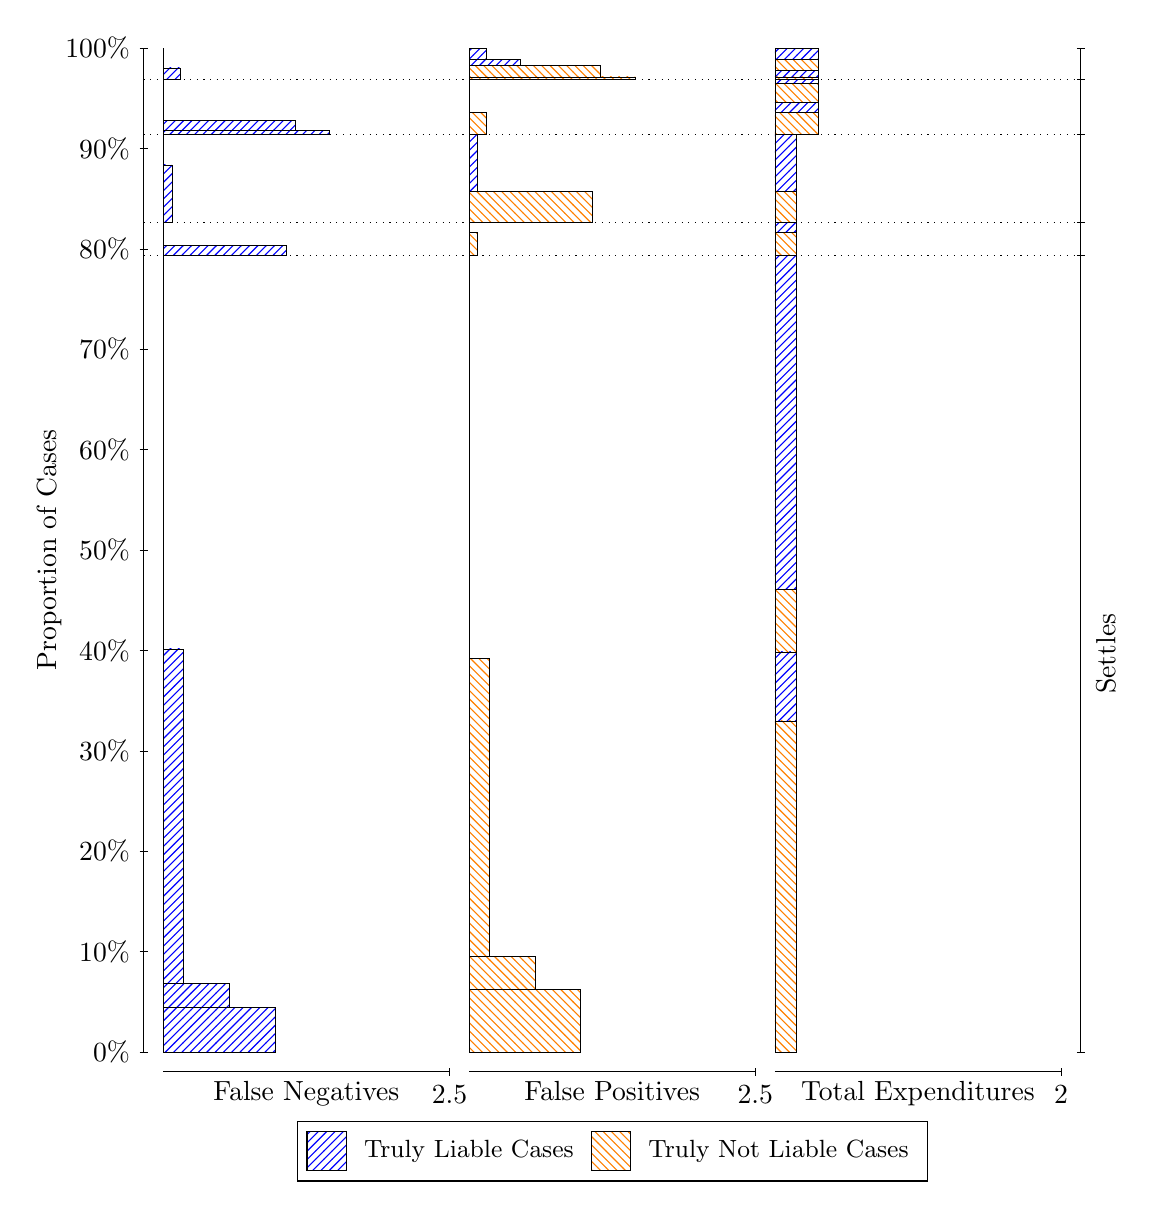
\begin{tikzpicture}
\draw[black, very thin] (1.5,1.75) -- (1.5,14.5);
\node[rotate=90, text=black, anchor=center] at (0.3, 8.125) {Proportion of Cases};
\draw[black, very thin] (1.45,1.75) -- (1.55,1.75);
\node[text=black, anchor=east] at (1.45, 1.75) {0\%};
\draw[black, very thin] (1.45,3.025) -- (1.55,3.025);
\node[text=black, anchor=east] at (1.45, 3.025) {10\%};
\draw[black, very thin] (1.45,4.3) -- (1.55,4.3);
\node[text=black, anchor=east] at (1.45, 4.3) {20\%};
\draw[black, very thin] (1.45,5.575) -- (1.55,5.575);
\node[text=black, anchor=east] at (1.45, 5.575) {30\%};
\draw[black, very thin] (1.45,6.85) -- (1.55,6.85);
\node[text=black, anchor=east] at (1.45, 6.85) {40\%};
\draw[black, very thin] (1.45,8.125) -- (1.55,8.125);
\node[text=black, anchor=east] at (1.45, 8.125) {50\%};
\draw[black, very thin] (1.45,9.4) -- (1.55,9.4);
\node[text=black, anchor=east] at (1.45, 9.4) {60\%};
\draw[black, very thin] (1.45,10.675) -- (1.55,10.675);
\node[text=black, anchor=east] at (1.45, 10.675) {70\%};
\draw[black, very thin] (1.45,11.95) -- (1.55,11.95);
\node[text=black, anchor=east] at (1.45, 11.95) {80\%};
\draw[black, very thin] (1.45,13.225) -- (1.55,13.225);
\node[text=black, anchor=east] at (1.45, 13.225) {90\%};
\draw[black, very thin] (1.45,14.5) -- (1.55,14.5);
\node[text=black, anchor=east] at (1.45, 14.5) {100\%};

\draw[black, very thin] (13.4,1.75) -- (13.4,14.5);
\draw[black, very thin] (13.35,1.75) -- (13.45,1.75);
\node[anchor=west] at (13.35, 1.75) {};
\draw[black, very thin] (13.35,11.866) -- (13.45,11.866);
\node[anchor=west] at (13.35, 11.866) {};
\draw[black, very thin] (13.35,12.289) -- (13.45,12.289);
\node[anchor=west] at (13.35, 12.289) {};
\draw[black, very thin] (13.35,13.406) -- (13.45,13.406);
\node[anchor=west] at (13.35, 13.406) {};
\draw[black, very thin] (13.35,14.102) -- (13.45,14.102);
\node[anchor=west] at (13.35, 14.102) {};
\draw[black, very thin] (13.35,14.5) -- (13.45,14.5);
\node[anchor=west] at (13.35, 14.5) {};

\draw[black, very thin, pattern color=blue, pattern=north east lines] (1.75,1.75) rectangle (3.167,2.32);
\draw[black, very thin, pattern color=blue, pattern=north east lines] (1.75,2.32) rectangle (2.5857,2.6245);
\draw[black, very thin, pattern color=blue, pattern=north east lines] (1.75,2.6245) rectangle (2.0043,6.8683);
\draw[black, very thin, pattern color=orange, pattern=north west lines] (1.75,6.8683) rectangle (1.75,11.866);
\draw[black, very thin, pattern color=blue, pattern=north east lines] (1.75,11.866) rectangle (3.3123,11.997);
\draw[black, very thin, pattern color=orange, pattern=north west lines] (1.75,11.997) rectangle (1.75,12.289);
\draw[black, very thin, pattern color=blue, pattern=north east lines] (1.75,12.289) rectangle (1.859,13.015);
\draw[black, very thin, pattern color=orange, pattern=north west lines] (1.75,13.015) rectangle (1.75,13.406);
\draw[black, very thin, pattern color=blue, pattern=north east lines] (1.75,13.406) rectangle (3.8573,13.454);
\draw[black, very thin, pattern color=blue, pattern=north east lines] (1.75,13.454) rectangle (3.4213,13.579);
\draw[black, very thin, pattern color=orange, pattern=north west lines] (1.75,13.579) rectangle (1.75,14.102);
\draw[black, very thin, pattern color=blue, pattern=north east lines] (1.75,14.102) rectangle (1.968,14.249);
\draw[black, very thin, pattern color=orange, pattern=north west lines] (1.75,14.249) rectangle (1.75,14.422);
\draw[black, very thin, pattern color=blue, pattern=north east lines] (1.75,14.422) rectangle (1.75,14.5);
\draw[black, very thin, pattern color=orange, pattern=north west lines] (5.6333,1.75) rectangle (7.0503,2.5418);
\draw[black, very thin, pattern color=orange, pattern=north west lines] (5.6333,2.5418) rectangle (6.469,2.967);
\draw[black, very thin, pattern color=orange, pattern=north west lines] (5.6333,2.967) rectangle (5.8877,6.7477);
\draw[black, very thin, pattern color=blue, pattern=north east lines] (5.6333,6.7477) rectangle (5.6333,11.866);
\draw[black, very thin, pattern color=orange, pattern=north west lines] (5.6333,11.866) rectangle (5.7423,12.158);
\draw[black, very thin, pattern color=blue, pattern=north east lines] (5.6333,12.158) rectangle (5.6333,12.289);
\draw[black, very thin, pattern color=orange, pattern=north west lines] (5.6333,12.289) rectangle (7.1957,12.68);
\draw[black, very thin, pattern color=blue, pattern=north east lines] (5.6333,12.68) rectangle (5.7423,13.406);
\draw[black, very thin, pattern color=orange, pattern=north west lines] (5.6333,13.406) rectangle (5.8513,13.683);
\draw[black, very thin, pattern color=orange, pattern=north west lines] (5.6333,13.683) rectangle (5.6333,13.928);
\draw[black, very thin, pattern color=blue, pattern=north east lines] (5.6333,13.928) rectangle (5.6333,14.102);
\draw[black, very thin, pattern color=orange, pattern=north west lines] (5.6333,14.102) rectangle (7.7407,14.134);
\draw[black, very thin, pattern color=orange, pattern=north west lines] (5.6333,14.134) rectangle (7.3047,14.275);
\draw[black, very thin, pattern color=blue, pattern=north east lines] (5.6333,14.275) rectangle (6.2873,14.353);
\draw[black, very thin, pattern color=blue, pattern=north east lines] (5.6333,14.353) rectangle (5.8513,14.5);
\draw[black, very thin, pattern color=orange, pattern=north west lines] (9.5167,1.75) rectangle (9.7892,5.9559);
\draw[black, very thin, pattern color=blue, pattern=north east lines] (9.5167,5.9559) rectangle (9.7892,6.8304);
\draw[black, very thin, pattern color=orange, pattern=north west lines] (9.5167,6.8304) rectangle (9.7892,7.6222);
\draw[black, very thin, pattern color=blue, pattern=north east lines] (9.5167,7.6222) rectangle (9.7892,11.866);
\draw[black, very thin, pattern color=orange, pattern=north west lines] (9.5167,11.866) rectangle (9.7892,12.158);
\draw[black, very thin, pattern color=blue, pattern=north east lines] (9.5167,12.158) rectangle (9.7892,12.289);
\draw[black, very thin, pattern color=orange, pattern=north west lines] (9.5167,12.289) rectangle (9.7892,12.68);
\draw[black, very thin, pattern color=blue, pattern=north east lines] (9.5167,12.68) rectangle (9.7892,13.406);
\draw[black, very thin, pattern color=orange, pattern=north west lines] (9.5167,13.406) rectangle (10.062,13.683);
\draw[black, very thin, pattern color=blue, pattern=north east lines] (9.5167,13.683) rectangle (10.062,13.809);
\draw[black, very thin, pattern color=orange, pattern=north west lines] (9.5167,13.809) rectangle (10.062,14.054);
\draw[black, very thin, pattern color=blue, pattern=north east lines] (9.5167,14.054) rectangle (10.062,14.102);
\draw[black, very thin, pattern color=orange, pattern=north west lines] (9.5167,14.102) rectangle (10.062,14.134);
\draw[black, very thin, pattern color=blue, pattern=north east lines] (9.5167,14.134) rectangle (10.062,14.212);
\draw[black, very thin, pattern color=orange, pattern=north west lines] (9.5167,14.212) rectangle (10.062,14.353);
\draw[black, very thin, pattern color=blue, pattern=north east lines] (9.5167,14.353) rectangle (10.062,14.5);
\draw[black, dotted] (1.5,11.866) -- (13.4,11.866);
\draw[black, dotted] (1.5,12.289) -- (13.4,12.289);
\draw[black, dotted] (1.5,13.406) -- (13.4,13.406);
\draw[black, dotted] (1.5,14.102) -- (13.4,14.102);
\draw[black, very thin] (1.75,1.5) -- (5.3833,1.5);
\node[text=black, anchor=north] at (3.5667, 1.5) {False Negatives};
\draw[black, very thin] (5.3833,1.45) -- (5.3833,1.55);
\node[text=black, anchor=north] at (5.3833, 1.45) {2.5};

\draw[black, very thin] (5.6333,1.5) -- (9.2667,1.5);
\node[text=black, anchor=north] at (7.45, 1.5) {False Positives};
\draw[black, very thin] (9.2667,1.45) -- (9.2667,1.55);
\node[text=black, anchor=north] at (9.2667, 1.45) {2.5};

\draw[black, very thin] (9.5167,1.5) -- (13.15,1.5);
\node[text=black, anchor=north] at (11.333, 1.5) {Total Expenditures};
\draw[black, very thin] (13.15,1.45) -- (13.15,1.55);
\node[text=black, anchor=north] at (13.15, 1.45) {2};

\node[text=black, centered, rotate=90] at (13.72, 6.808) {Settles};





\draw (7.449999999999999,1.5) node[draw=none] (baseCoordinate) {};
\begin{scope}[align=center]
        \matrix[scale=0.5, draw=black, below=0.5cm of baseCoordinate, nodes={draw}, column sep=0.1cm]{
            \node[rectangle, draw, minimum width=0.5cm, minimum height=0.5cm, pattern color=blue, pattern=north east lines] {}; &
            \node[draw=none, font=\small, text=black] (B) {Truly Liable Cases}; &
            \node[rectangle, draw, minimum width=0.5cm, minimum height=0.5cm, pattern color=orange, pattern=north west lines] {}; &
            \node[draw=none, font=\small, text=black] (B) {Truly Not Liable Cases}; \\
            };
\end{scope}

\end{tikzpicture}
\end{document}